\section{Relações de recorrência}
\

Na sessão anterior, o pseudocódigo para o algoritmo fatorial recursivo foi apresentado. Através dele, é observável que a solução para $a_r = r! \ (r \in \mathbb{N})$, tendo como \textbf{condição inicial} $a_0 = 1$, pode ser computada através do que é chamado de \textbf{relação de recorrência}, nesse caso $a_r = ra_{r-1}$. Em uma \textbf{função definida recursivamente}, dado uma condição inicial e uma descrição dos estágios subsequentes em função dos anteriores é possível avaliar estágios da função para um dado $n$. Se $f$ for definida recursivamente, então $f(n)$ é única para qualquer inteiro positivo $n$.

A \textbf{solução de uma relação de recorrência} é uma expressão que de o valor da função em termos de seus argumentos e que não dependa de sub expressões. Não existe um método geral para solucionar uma relação de recorrência arbitrária. Existem classes de relações de recorrência onde técnicas de solução são conhecidas.

Por vezes, encontrar a solução da recorrência é difícil e é possível contentar-se apenas com uma boa estimativa assintótica da cota superior.

\subsection{Método da substituição}
\

O método da substituição é capaz de resolver recorrências simples, basta escrever os termos em função de seus antecessores e assim dar um palpite sobre a forma geral solucionando a recursão.

\textbf{Exemplo 1}

Uma simples relação de recorrência, $a_n = a_{n-1} + 1$ e $a_0=0$ pode ter uma solução encontrada por substituição de alguns termos.
\[a_n = a_{n-1} + 1 \Rightarrow a_{n-1} = a_{n-2} + 1 \Rightarrow a_n = a_{n-2} + 2\]
\[a_n = a_{n-k} + k\]

Assumindo $k=n$ temos que $a_n=a_0 + n$ pois $n-k = 0$, como $a_0=0$, então $a_n=n$ é a solução da recorrência. Por último, a notação $T(n)=T(n-1)+1$ e $T(0)=0$ com solução $T(n) = n$ é frequentemente utilizada, é claro que $T(n) \in O(n)$.

{\raggedleft $\bigtriangleup$ \par}

\textbf{Exemplo 2}

Para encontrar a solução de $a_n = a_{n-1} + n + 1$ com $a_0 = 0$ também é possível reescrever $a_n$
\[a_n = a_{n-1} + n + 1 = (a_{n-2} + (n-1) + 1) + n + 1 = a_{n-2} + (n-1) + n + 2 = a_{n-3} + (n-2) + (n-1) + n + 3\]

\[a_n = a_{n-k} + (n-k+1) + ... + (n-1) + n + k\]

Supondo $k=n$

\[a_n = a_0 + 1 + ... + (n-1) + 2n = \frac{n(n+1)}{2} + n \in O(n^2).\]

{\raggedleft $\bigtriangleup$ \par}

\textbf{Exemplo 3}

Resolva a recorrência $a_n = a_{n/2} + n$ com $a_0 = 1$, note que faz sentido falar de $n$ apenas no conjunto de potências de $2$, logo $n=2^k$. Usando a notação $T(n)=T(2^k)$.

\[T(n) = T \Bigr(\frac{n}{2}\Bigr) + n = \Bigr[T\Bigr(\frac{n}{2^2}\Bigr) + \frac{n}{2}\Bigr] + n\]
\[T(n) = T\Bigr(\frac{n}{2^k}\Bigr) + \frac{n}{2^k} + ... + \frac{n}{2} + n\]

Fazendo $k=\log_2(n)$

\[T(n) = T(1) + n\sum_{i=1}^k \frac{1}{i} = 1 + 2n \in O(n).\]

{\raggedleft $\bigtriangleup$ \par}

\subsection{Teorema mestre para funções decrescentes}
\

A seguir são apresentadas as soluções (sugestão de exercício) assintóticas para algumas relações de recorrência. A partir da observação, podemos conjecturar uma forma geral de solução assintótica a ser seguida.
\[T(n)=T(n-1)+1 \in O(n);\]
\[T(n)=T(n-1)+n \in O(n^2);\]
\[T(n)=T(n-1)+ \log n \in O(n \log n);\]
\[T(n)=2T(n-2)+1 \in O(2^{\frac{n}{2}});\]
\[T(n)=3T(n-1)+1 \in O(3^n);\]
\[T(n)=2T(n-1)+n \in O(n2^n).\]

Uma conjectura apropriada, que pode ser demonstrada como teorema mestre para funções decrescentes é que para uma relação de recorrência da forma $T(n)=aT(n-b)+f(n)$, com $a>0$, $b>0$ e sendo $f(n)=O(n^k)$ onde $k\geq 0$, existem três soluções assintóticas que podem ser sumarizadas

(1) Se $a<1$ então $T(n) \in O(n^k)$ ou ainda $T(n) \in O(f(n))$;

(2) Se $a=1$ então $T(n) \in O(n^k+1)$ ou ainda $O(nf(n))$;

(3) Se $a>1$ então $T(n) \in O(n^ka^{\frac{n}{b}})$ ou ainda $O(f(n)a^{\frac{n}{b}})$.

\subsection{Teorema mestre}
\

Sejam $a\geq 1$ e $b>1$ constantes, $f(n)$ uma função e $T(n)$ definida em $\mathbb{N}_0$ pela recorrência $T(n) = aT\Bigr(\frac{n}{b}\Bigr) + f(n)$, $T(n)$ tem os seguintes limites assintóticos

(1) Se $f(n) \in O\Bigr(\frac{n^{\log_ba}}{n^\epsilon}\Bigr)$ para alguma constante $\epsilon>0$, então $T(n) \in \Theta(n^{\log_ba})$;

(2) Se $f(n) \in \Theta(n^{\log_ba})$, então $T(n) \in \Theta(n^{\log_ba} \log n)$;

(3) Se $f(n) \in \Omega(n^{\log_ba}n^\epsilon)$ para alguma constante $\epsilon>0$ e $ \ \exists c; \ af\Bigr(\frac{n}{b}\Bigr)\leq cf(n) $ então $T(n) \in \Theta(f(n))$.


O Teorema mestre dá a solução assintótica para recorrências da forma $aT\Bigr(\frac{n}{b}\Bigr) + f(n)$. Muitas vezes saber a ordem de crescimento da recorrência já é suficiente e uma solução de fórmula fechada não é necessária.

De modo intuitivo, o teorema mestre que ao comparar $f(n)$ e $n^{\log_ba}$ o caso (1) ocorre se $f(n)$ for polinomialmente menor que $n^{\log_ba}$, no caso (2) se forem iguais e no caso (3) se $f(n)$ for polinomialmente maior que $n^{\log_ba}$. Como essa diferença por um fator polinomial $n^\epsilon$ é obrigatória existem classes de funções $f(n)$ que são menores que $n^{\log_ba}$ mas não polinomialmente menores, dessa forma, o primeiro caso do teorema mestre não se aplicaria, isso é análogo para o terceiro caso.

\textbf{Exemplo 1}

$T(n)=9T\Bigr(\frac{n}{3}\Bigr) + n$. Primeiramente, identificando os termos se obtém, $a=9$, $b=3$ e $f(n)=n$.

Em segundo lugar, avaliando $n^{\log_ba}=n^{\log_3 9} = n^2$. Tomando $\epsilon = 1$, $f(n) = O(n^{2-1})$ e $f(n) = n \prec n^2$, o primeiro caso é satisfeito e $T(n) \in \Theta(n^2).$

{\raggedleft $\bigtriangleup$ \par}

\textbf{Exemplo 2}

$T(n) = 2T\Bigr(\frac{n}{4}\Bigr) + \sqrt{n}$. Para essa recorrência, $a = 2$, $b = 4$ e $f(n) = \sqrt{n}$, ao avaliar $n^{\log_ba}=n^{\log_4 2} = \sqrt{n}$. Como $f(n) = \Theta(\sqrt{n})$ o segundo caso é satisfeito e $T(n) \in \Theta(\sqrt{n}\log n)$.

{\raggedleft $\bigtriangleup$ \par}

\textbf{Exemplo 3 (Teorema não se aplica)}

$T(n) = 6T\Bigr(\frac{n}{6}\Bigr) + {n \log n}$. Neste caso $n^{\log_ba} = n \prec n \log n$, entretanto, o terceiro caso não se aplica, observando que $f(n)$ não é polinomialmente maior que $n$, é apenas maior por um fator $\log n$.

{\raggedleft $\bigtriangleup$ \par}

\textbf{Exemplo 4}

$T(n) = 3T\Bigr(\frac{n}{4}\Bigr) + {n \log n}$. Identificando os termos na recorrência, $n^{\log_4 3} = n^{0,793}$. Para uma constante $\epsilon \approx 0,2$, $f(n) = \Omega(n^{0,793}n^{0,2})$. Verificando a condição de regularidade $af\Bigr(\frac{n}{b}\Bigr) = 3\Bigr(\frac{n}{4}\Bigr)\log\Bigr(\frac{3}{4}\Bigr) \leq \Bigr(\frac{3}{4}\Bigr) n \log n \leq \frac{3}{4}f(n)$ logo $c=\frac{3}{4}$. Assim, o terceiro caso do teorema mestre pode ser aplicado e $T(n) \in \Theta (n \log n)$.

{\raggedleft $\bigtriangleup$ \par}

\subsection{Algoritmos recursivos}
\

Uma relação de recorrência é uma fórmula recursiva. Um procedimento recursivo na ciência da computação, chama a si próprio para resolver um problema similar porém menor, se a instância é pequena, ele a resolve diretamente como puder. Um exemplo de algoritmo recursivo é o de computar a soma dos números de Fibonacci até uma indexação $n$.

\begin{lstlisting}[language=C, frame=single]
    int fibonacci(n)
    {
        if(n <= 1) return n

        else return fibonacci(n-1) + fibonacci(n-2)
    }
\end{lstlisting}

Na sessão anterior, fora apresentado, com poucos detalhes, um algoritmo, sem muita utilidade, que fazia chamadas de forma a configurar uma complexidade exponencial $O(2^n)$. Observando o algoritmo recursivo de Fibonacci, é fácil notar que o tempo de uma chamada depende de outras duas e que \texttt{return} em \texttt{if} tem complexidade $k \in O(1)$, obtendo uma complexidade

\[T(n) = T(n-1) + T(n-2) + O(1).\]

A chamada \texttt{fibonacci(n-1)} faz mais chamadas subsequentes do que a chamada \texttt{fibonacci(n-2)}, entretanto, assumindo que as duas chamadas a mais são, por hora, irrelevantes é possível dizer que $T(n-1)\approx T(n-2)$ e encontrar uma cota assintótica superior pelo método da substituição. Os casos base $T(0)$ e $T(1)$ tem complexidade de tempo de execução constante.

\[T(n-1)\approx T(n-2) \Rightarrow T(n) = 2T(n-1) + k = 2[2T(n-2)+k]+k = 4T(n-2) + 3k\]
\[T(n) = 2^r[T(n-r)]+(2^{r}-1)k.\]

Fazendo em $T(0)=T(1)=1$, o termo $T(n-r)=T(0)$ leva a $n=r$. $T(n) = 2^n + (2^n-1)k \in O(2^n)$. Logo o limite assintótico da cota superior é exponencial.

Um fato interessante é que a relação de recorrência encontrada no momento do cálculo de complexidade $T(n)=T(n-1)+T(n-2)+O(1)$ se assemelha bastante a relação de recorrência da própria função de Fibonacci $a_n=a_{n-1}+a_{n-2}$. Em uma próxima sub sessão será apresentado um método capaz de encontrar uma solução $g(n)$ para o termo geral da série de Fibonacci que tem o termo mais significativo $\Bigr(\frac{1+\sqrt{5}}{2}\Bigr)^n < 2^n$. Sabendo que se $a<b$ então $a^n \in O(b^n)$ então é possível dizer $a_n \in O(1,62^n) \subset O(2^n)$. Embora a relação de recorrência encontrada na resolução da complexidade seja similar a usada para encontrar o termo geral de Fibonacci, elas não são a mesma recorrência.

\subsubsection{Método da árvore de recursão para resolução de relações de recorrências}
\

A complexidade do algoritmo recursivo de Fibonacci pode ter uma solução assintótica a partir do \textbf{método da árvore de recursão}. O método consiste em atribuir a cada nó um custo de um subproblema dentro do conjunto de chamadas da função recursiva e pode ser aplicado quando for difícil um palpite sobre a forma no método da substituição por exemplo.

Na árvore de recursão para o algoritmo recursivo de Fibonacci, o custo de uma função dependera das próximas chamadas e observamos o crescimento de uma árvore binária. A figura 6 ilustra um diagrama da árvore de recursão. Note que a quantidade de chamadas aproxima-se de $2^n$, encontrando uma cota superior para a complexidade.

\begin{figure}
  \centering
  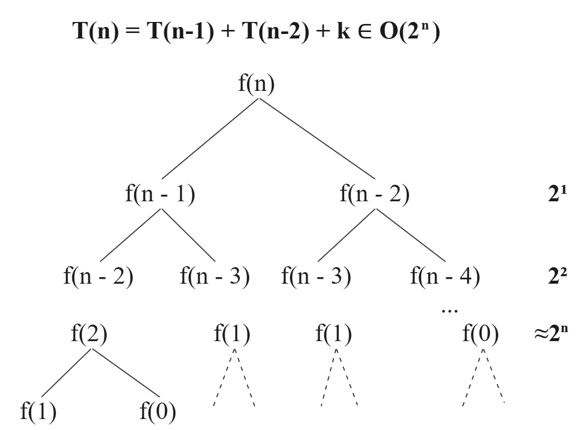
\includegraphics[width=0.7\linewidth]{img/arvorerecursaofib.png}
    \caption{Árvore de recursão para o algoritmo recursivo de Fibonacci.}
    \label{arvorerecursaofib}
\end{figure}

\subsection{Divisão e conquista}
\

Relembrando alguns tópicos, uma relação de recorrência é recursiva. Um algoritmo com procedimento recursivo resolve uma instância pequena como pode, reduz instância grandes a menores e após resolvidas retorna as originais, essa característica de trabalhar para trás é muito comum.

A \textbf{divisão e conquista} é uma estratégia para desenvolver algoritmos, com uma definição similar a apresentada para algoritmos recursivos. A técnica de divisão e conquista, frequentemente mais eficiente que métodos de força bruta para a resolução de problemas algorítmicos consiste em algumas etapas.

Primeiramente, o problema geral é \textbf{dividido} em problemas não sobrepostos de tamanhos aproximadamente iguais, esses subproblemas são instâncias menores do problemas geral. Em segundo lugar, ocorre a etapa de \textbf{conquista}, que consiste em solucionar recursivamente os subproblemas. Por último, os subproblemas são \textbf{combinados} solucionando o problema geral.

Dentre os algoritmos que seguem essa estratégia estão o \texttt{algoritmo numérico da bisseção}, os algoritmos de ordenação \texttt{quicksort} e \texttt{mergesort} onde a estratégia é bastante explicita e o algoritmo para multiplicação de matrizes de \texttt{Strassen} que reduz a complexidade do algoritmo ingenuo.

\textbf{Exemplo (Busca binária)}

A busca binária é um algoritmo para encontrar um valor em um vetor ordenado. O algoritmo consiste em buscar sempre o valor no meio do vetor, como este está ordenado, caso o valor procurado seja menor que o palpite, o algoritmo reduz a busca apenas a metade a esquerda do valor, o mesmo ocorre se o valor for maior, mas com a metade a direita. O problema então tem seu tamanho dividido, aproximadamente, pela metade do tamanho original sucessivamente, a complexidade do tempo de execução da busca binária, \texttt{binary\_search}, está em $O(\log n)$.

\begin{figure}
  \centering
  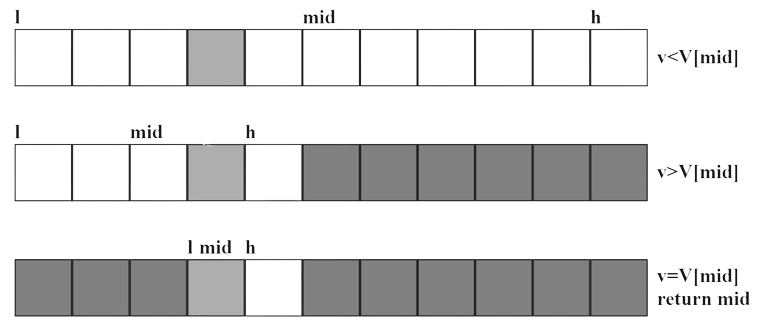
\includegraphics[width=1\linewidth]{img/binary_search.png}
    \caption{Diagrama de representação da busca binária, os elementos em cinza escuro são os eliminados do vetor a medida que o algoritmo é executado}
    \label{binary_search}
\end{figure}

No pseudocódigo abaixo, \texttt{v} é o valor procurado, \texttt{h} e \texttt{l} indicam as extremidades do vetor, que será dividido em sub vetores.

\begin{lstlisting}[language=C, frame=single]
    int binary_search(l,h,v,V)
    {
        if(h==l)
        {
            if(V[l]==v) return v
            else return (-1)
        }
        
        else
        {
            mid = (l+h)/2
            if(v==V[mid]) return mid
            if(v<V[mid]) return binary_search(l, mid-1, v)
            else return(mid+1, h, v)
        }
    }
\end{lstlisting}

Chamando de $T(n)$ a complexidade de tempo de execução da busca binária. O caso base da recursão está em $O(1)$ e as chamadas de subproblemas são $T\Bigr(\frac{n}{2}\Bigr)$. A solução assintótica da relação de recorrência $T(n)=T\Bigr(\frac{n}{2}\Bigr)+1$ pode ser obtida a partir do \textbf{teorema mestre}.

Tem-se que $a=1$, $b=2$, $f(n)=n^0=1$ e $n^{\log_2 1}=n^0$. Tendo em vista que $f(n)=n^0=1 \in \Theta(1)=\Theta(n^{\log_2 1})$, o segundo caso do teorema mestre se aplica e $T(n) \in \Theta(1 \log n)$ portanto

\[T(n) \in (\log n).\]



\subsection{Relações de recorrência homogêneas e não homogêneas}
\

O método da substituição pode ser difícil para algumas relações de recorrência e o método mestre é restrito para formatos de relações. Ainda existem classes que podem ser solucionadas de outras formas, similares a encontrar soluções para equações diferenciais simples.

Através dos métodos a seguir é possível solucionar recorrências como as somas de quadrados ou até mesmo a famosa sequência de Fibonacci.

\subsubsection{Princípio da superposição}
\

Se funções $g_i(n) (i = 1, ..., k)$ forem soluções para uma relação de recorrência linear com coeficientes constantes de ordem r, então a combinação linear das $k$ soluções, $A_1g_1(n) + ... + A_kg_k(n)$, é solução da relação de recorrência, $A_i \in \mathbb{R}$.

\subsubsection{Relações de recorrência homogêneas}
\

Uma \textbf{relação de recorrência linear com coeficientes constantes de ordem r} é definida como uma relação de recorrência da forma $a_n = k_1a_{n-1}+...+k_ra_{n-r} + f(n)$ sendo $k_i \ (i = 1, ... , r)$ constantes e $f(n) = 0$. Se $g(n)$ é uma função onde $a_n=g(n)$ então $g(n)$ é chamada de \textbf{solução} da relação de recorrência.

Digamos que $a_r = x^r$ é solução da relação, então $x^n = k_1x^{n-1}+...+k_rx^{n-r}$, e ignorando a solução trivial $x=0$, obtém-se a equação polinomial de grau $r$, $x^n - k_1x^{n-1}-...-k_rx^{n-r} = 0$, chamada de \textbf{equação característica} da relação de recorrência.

Se as raízes da equação características forem todas \textbf{reais e distintas}, a solução homogênea será da forma
\[a_n = A_1(x_1)^n + ... + A_n(x_n)^n.\]

\textbf{Exemplo 1}

$T(n) = 9T(n-2); \ T(0) = 6,  \ T(1) = 12$. Obtendo a equação característica, $x^2 - 9 = 0$, as raízes são avaliadas em $x_i = {-3,3}$. A solução da relação de recorrência é da forma $T(n) = A_1(-3)^n + A_2(3)^n$. Dadas as condições iniciais, $A_1 + A_2 = 6$ e $-3A_1 + 3A_2 = 12$, assim a solução é 
\[T(n) = (-3)^n + 5(3)^n.\]

\textbf{Exemplo 2 (Termo geral da sequência de Fibonacci)}

A sequência de Fibonacci com relação de recorrência $a_n = a_{n-1} + a_{n-2}$ com $a_0 = a_1 = 1$, pode ter uma solução obtida através do método apresentado.

As raízes da equação característica $x^2 - x - 1 = 0$ são $x_1 = \frac{1+\sqrt{5}}{2}$ e $x_2 = \frac{1 - \sqrt{5}}{2}$.

Usando a forma $a_n = A_1(x_1)^n + A_2(x_2)^n$, e as condições iniciais, avalia-se $A_1 = \frac{1 + \sqrt{5}}{2\sqrt{5}}$ e $A_2 = \frac{\sqrt{5} - 1 }{2\sqrt{5}}$.

Dessa forma, multiplicando os termos, a solução para a relação de recorrência de Fibonacci é 

\[\frac{\Bigr(\frac{1+\sqrt{5}}{2}\Bigr)^n-\Bigr(\frac{1 - \sqrt{5}}{2}\Bigr)^n}{\sqrt{5}}.\]

{\raggedleft $\bigtriangleup$ \par}

Caso as raízes apresentarem \textbf{multiplicidade}, sendo reais, ou seja, \textbf{reais e repetidas}, o formato de solução para raízes reais e distintas não funcionará mais pois ele violaria o princípio da superposição da combinação linear.

Se $x$ for uma raiz de multiplicidade então a solução particular será da forma

\[u_p = (x)^n(A_1 + ... + A_{k}x^{k-1}).\]

\textbf{Exemplo 3}

Se $x_1 = 2$ tiver multiplicidade $3$ e $x_2 = 6$ multiplicidade $2$ e ambas forem raízes de uma mesma equação característica então o formato da solução será

\[a_n = 2^n(A_1 + A_2n + A_3n^2) + 6^n(B_1n + B_2n^2).\]

{\raggedleft $\bigtriangleup$ \par}

\subsubsection{Relações de recorrência não homogêneas}

Quando uma relação de recorrência é do formato $a_n = h_n + f(n)$ com $f(n) \neq 0$, dizemos que $h_n$ é a \textbf{parte homogênea} da relação de recorrência não homogênea. A solução geral será a soma da solução da parte homogênea com a solução não homogênea.

Existem dois casos especiais onde técnicas de solução são conhecidas. Primeiramente, o caso onde $f(n) = k(q)^n$, onde $q \neq 1$ é um número racional e $k$ uma constante conhecida. A escolha para uma solução particular é $u_n = A(q)^n$, a menos que a $q$ seja uma raiz da equação característica, nesse caso a escolha seria $u_n = A(n)^r(q)^n$, onde $r$ é a multiplicidade da raiz.

O segundo caso é quando $f(n) = k(n)^r$, se a equação característica não possuir raiz $x = 1$, a solução é do formato $A_1 + ... + A_k(n)^{k-1}$. Se $1$ for uma raiz de multiplicidade $r$ então a escolha será $A_1n^t + ... + A_kn^{t+(k-1)}$.

\textbf{Exemplo (Soma de quadrados)} 

Avaliar a soma dos quadrados dos $n$ primeiros inteiros positivos.

A relação de recorrência é dada por $a_n = a_{n-1} + n^2$ com $a_0 = 0$. A solução homogênea é calculada como $x = 1$, de multiplicidade $1$, então a solução será da última forma apresentada.

A escolha para a solução particular não homogênea é $A_1n + A_2n^2 + A_3n^3$. Como $a_0 = 0$ a solução é da forma.

\[a_n = A_1n + A_2n^2 + A_3n^3,\]
\[a_n  = A_1(n-1) + A_2(n-1)^2 + A_3(n-1)^3 + n^2.\]

Colando os termos $n$ e $n^2$ em evidencia, um sistema pode ser formado para calcular $A_1 = \frac{1}{6}$, $A_2 = \frac{1}{2}$ e $A_3 = \frac{1}{3}$.

Dessa forma a solução é $a_n = \frac{n}{6} + \frac{n^2}{2} + \frac{n^3}{3}$, chegando no resultado

\[\sum_{i=1}^{n} i^2 = \frac{n(n+1)(2n+1)}{6}.\]

{\raggedleft $\bigtriangleup$ \par}
